\section{Waves}


%Introduction

%\subsection{String Waves}
%\begin{itemize}
%\item{Preparation time: none}
%\item{Materials: at least 2 meters of string}
%\item{Procedure: We can show several different types of waves using just a string. First, lay the string out along a table. By snapping your hand, you can create a transverse pulse wave that will travel along the length of the string. Now tie one end of the string to a rigid object and repeat. You should see the pulse reflect from the fixed end and come back towards you. Now wave the string up and down so as to create a standing wave. By changing the frequency with which you move your hand, you should be able to create at least two different modes.}
%\end{itemize}


\subsection{Construction and Use of Slinky Spring}

\subsubsection*{Learning Objectives}
\begin{itemize}
\item{To construct a slinky spring} 
\item{To observe the propagation of transverse and longitudinal waves} 
\end{itemize}

\subsubsection*{Background Information}
A mechanical wave is the oscillation of particles in a medium, either side-to-side or back-and-forth along the direction of the wave's motion. A transverse mechanical wave is produced when particles oscillate side-to-side as on a guitar string. Its crests and troughs can be seen clearly. A longitudinal wave is produced when particles oscillate back-and-forth as passengers on a bus that stops and starts repeatedly. It can be seen because of the alternating compressions and rarefactions along the wave.  

\subsubsection*{Materials}
Two (2) m of flexible steel or copper wire, long cylindrical object (rod, stick) at least 3 cm diameter

\subsubsection*{Hazards and Safety}
\begin{itemize}
\item{Every spring has a maximum length that it can be stretched. If you stretch it beyond this point, it will not work again. Don't stretch the slinky too far.} 
\end{itemize}

\subsubsection*{Preparation Procedure}
\begin{enumerate}
\item{Collect all materials.} 
\item{Hold one end of the wire against the cylindrical object.} 
\item{Use your other hand to coil the wire around the cylinder, keeping the coils close together. When you finish coiling all of the wire along the cylinder, you should have a slinky spring.} 
\end{enumerate}

\subsubsection*{Activity Procedure}
\begin{enumerate}
\item{Have one student hold one end of the spring.} 
\item{Hold the other end with your hand and stretch the slinky slightly so that the coils separate.} 
\item{Hold the slinky flat against the floor.} 
\item{Move your end of the slinky quickly from side to side (the student should keep her end stationary). Observe the motion of the slinky.} 
\item{Move your hand quickly back and forth, alternately pushing and pulling the spring. Observe the motion of the slinky.} 
\item{Move your hand quickly to one side and then back to the center only once. Observe the progression of the wave along the slinky.} 
\end{enumerate}

\subsubsection*{Results and Conclusions}
Students will see that a transverse wave progresses by alternating crests and troughs as the points on the slinky oscillate back and forth perpendicular to the direction of the wavefront.  
Students will see that a longitudinal wave progresses as points on the slinky alternately push and pull each other in the direction of the wavefront.  
Students will see that a single transverse wave (one crest and one trough) is reflected on the opposite side, or that the crest and trough trade places when reflected.  
Students should understand that a wave is caused when particles oscillate.  

\subsubsection*{Clean Up Procedure}
Return the slinky to its proper place.

\subsubsection*{Discussion Questions}
\begin{enumerate}
\item{What is the type of wave produced when you move your hand from side to side? Describe this wave.} 
\item{What is the type of wave produced when you move your hand back and forth? Describe this wave.} 
\item{When there is only one wave crest moving along the slinky, how is it reflected at the opposite end?}
\end{enumerate}


\subsection{Speed of Sound in Air}

\subsubsection*{Learning Objectives}
\begin{itemize}
\item{To understand the relationship between a wave's frequency, speed and wavelength} 
\item{To calculate the speed of sound in air using a resonance tube} 
\end{itemize}

\subsubsection*{Background Information}
A wave's speed or velocity is directly related to the wave's frequency and wavelength. If the wavelength and frequency can be determined, the speed can be calculated easily. We can use a resonance tube or sonometer to find the wavelength and frequency of a wave, therefore allowing us to calculate the speed of the sound wave in that medium.  

\subsubsection*{Materials}
Resonance tube (this can be made: see the activity about constructing a resonance tube in this book), tuning fork or wind instrument like a flute or recorder, water, metre rule

\subsubsection*{Hazards and Safety}
\begin{itemize}
\item{If you are using tuning forks, do not hit them on a table or any other hard object. Over time, this will damage the tuning forks and changes their frequencies until they are no longer useful. Instead, hold the middle of the handle and hit one of the fork's prongs on the sole of your shoe or any other hard rubber object.} 
\end{itemize}

\subsubsection*{Preparation Procedure}
\begin{enumerate}
\item{Set up the resonance tube with water.} 
\item{Place the metre rule next to the resonance tube so that the 0 cm mark is at the top of the resonance tube.} 
\end{enumerate}

\subsubsection*{Activity Procedure}
\begin{enumerate}
\item{Use a tuning fork or flute to make a single musical note.} 
\item{Place the fork or flute over the resonance tube and adjust the water level until the resonance can be heard in the tube. The note produced by the fork or flute will be heard at the top of the tube when the water is at a certain level.} 
\item{Record the distance between the water level and the top of the tube at the level when the water reaches a level where resonance can be heard.} 
\item{Also record the frequency of the note. If you are using tuning forks, the frequency is written on the handle. If you are using a flute, the frequency depends on the note you are playing. A table of musical notes and their frequencies can be found in any textbook. The easiest to use is A, which has a frequency of 440 Hz.} 
\item{Use your values of length (wavelength) and frequency to calculate the speed of sound in the tube.} 
\item{Repeat these steps for several notes and compare your values of speed of sound.} 
\end{enumerate}

\subsubsection*{Results and Conclusions}
It will be seen that the product of wavelength and frequency will be almost the same. This is because the speed of sound in air is constant (depending on humidity and density). Therefore, the product of wavelength and frequency must be constant. As frequency increases, the wavelength (the length of the tube above the water level) decreases.  

\subsubsection*{Clean Up Procedure}
\begin{enumerate}
\item{Empty the water from the resonance tube.} 
\item{Return all materials to their proper places.} 
\end{enumerate}

\subsubsection*{Discussion Questions}
\begin{enumerate}
\item{What was your average value for the speed of sound in air?}
\item{As the frequency of the musical note increased, did its wavelength increase or decrease?}
\item{If the speed of a wave remains constant, what is the relationship between wavelength and frequency of a wave?}
\end{enumerate}

\subsubsection*{Notes}
There is room for error in this experiment because you are trying to measure length as the water level is moving. Also, the flute or other instrument you are using to create a note may not be perfectly in tune and so may have a slightly different frequency. Do several experiments in order to find a consistent value for the wavelength.



\subsection{Bottle Sine Graph}
\begin{itemize}
\item{Preparation time: 5 minutes}
\item{Materials: Empty water bottle, string (approximately 0.5m), water}
\item{Construction: Remove the cap of a water bottle and make a small hole in the center of the bottom with a syringe needle or a nail. Tie a string around the top of the water bottle.}
\item{Procedure: Fill the water bottle. Swing it as a pendulum from left to right while walking forwards. Water will pour out from the bottom of the water bottle in a thin stream, leaving a wet mark on the floor, which creates a graph of its position.}
\item{Theory: As you walk forward, you cause the forward direction to be the time axis. The bottle swings left to right, leaving a watery record of where it has been. Because a swinging pendulum executes simple harmonic motion, this demonstration allows us to see that simple harmonic motion has the shape of a sine curve.}
\end{itemize}


%Behaviour of Waves (Ripple Tank)

%\subsection{Ripple tank}
%\begin{itemize}
%\item{Preparation time: 1-2 hours}
%\item{Materials: pane of glass (40 cm x 60 cm is average), wood frame, caulk or some sealant, straight-edge, pen, lamp or torch, white paper.}
%\item{Construction: Make the ripple tank itself using an old window in its frame, or have a craftsman make a sealed window to your specifications (bigger is better, but use what is available). Seal the glass and frame with caulk or some equivalent so that water will not leak through it. Prop this shallow tank up on stands or books about a foot off the table; place the lamp above the tank facing straight down and the paper about 30 cm directly below the tank.}
%\item{Procedure: Level the tank and fill it with water 5 mm deep. Turn on the lamp so that any variation in the water’s surface shows up as a shadow on the white paper underneath. Create plane waves using a ruler or circular waves using a pen. You can also attach a thin strip of metal so that half hangs over the tank and half outside. Attach a pen to the inside half and flick the metal strip. If the masses on either side of the tank frame are equal, the strip should oscillate fairly easily. Observe diffraction, reflection, etc. by placing objects in the tank. All phenomena will be visible on the paper and can be measured there.}
%\item{Theory: Water waves, while different from sound or light waves, show the same properties of propagation, reflection, diffraction, etc. as any other wave. The varying depth of the water due to oscillating crests and troughs creates areas of bright and dark spots from the lamp above. Any behavior of the waves can be seen clearly and even measured: wavelength, frequency, and wave velocity.}
%\end{itemize}


\subsection{Construction of a Ripple Tank}

\subsubsection*{Learning Objectives}
\begin{itemize}
\item{To construct a ripple tank} 
\end{itemize}

\subsubsection*{Background Information}
A ripple tank uses a container or shallow water to create waves and observe their behavior. A light source projects the shadow of the waves onto the paper below so that all behavior at obstacles and sources can be seen clearly.

\subsubsection*{Materials}
pane of glass 45 cm by 45 cm, four pieces of wood 50 cm long and 4 cm thick, nails or screws, putty or caulk, small ball of plastic or rubber, stiff wire, small motor from a car stereo or other device, connecting wires, two D-cell batteries, four thin pieces of wood about 30 cm long, two thin pieces of wood about 50 cm long, various small pieces of straight wood, glue


\subsubsection*{Preparation Procedure}
\begin{enumerate}
\item{Obtain the 45 cm x 45 cm piece of glass.} 
\item{Make a groove 1 cm thick along one side of each of the four pieces of wood.} 
\item{From the groove on each piece of wood, cut the wood back at a 45-degree angle.} 
\item{Fit the pane of glass into the grooves and join the pieces of wood at the corners with nails or screws. It should resemble a window frame.} 
\item{Use caulk or putty to secure the glass to the wood frame so that water cannot pass.} 
\item{Make or find a small ball of rubber or plastic (no more than 2 cm diameter).} 
\item{Bend a 6 cm piece of wire into an L shape.} 
\item{Attach one end of the wire to the small ball.} 
\item{Along two opposite sides of the frame, attach two pieces of wood 30 cm tall vertically. These should be about 10 cm from the side and directly across from each other.} 
\item{Attach the two vertical pieces of wood at the top with the 50 cm piece of wood. You should now have a beam across the ripple tank.} 
\item{Attach the motor to a piece of wood 30 cm long. Try to balance the motor so that the piece of wood stays flat.} 
\item{Attach the ball and wire to one side of the piece of wood just under the motor. If the wood is flat, the wire should extend out and down.} 
\item{Suspend the wood and motor from the beam with thread so that the ball rests about 1 cm above the glass pane.} 
\item{Connect the terminals of the motor to connecting wires and extend these wires up to the beam.} 
\item{Attach two D-cell batteries to the beam so that the connecting wires can be easily attached.} 
\item{Glue a screw to the motor so that it vibrates when it spins.} 
\end{enumerate}

\subsubsection*{Activity Procedure}
Set up the ripple tank with water, a light source and plane paper to check that it works.

\subsubsection*{Results and Conclusions}
The motor on the hanging bar provides a vibration, which in turn produces waves in the water.  Different objects can be attached to the hanging bar to produce different types of waves, and the waves can be seen clearly on the paper under the tank. 

\subsubsection*{Clean Up Procedure}
\begin{enumerate}
\item{Disconnect the wires.} 
\item{Remove the water from the ripple tank.} 
\item{Return all materials to their proper places.} 
\end{enumerate}

\subsubsection*{Discussion Questions}
\begin{enumerate}
\item{Why is it necessary to attach an object to the motor?}
\item{What is the shape of a wave produced by the ball?}
\item{What is the shape of a wave produced by a ruler?}
\end{enumerate}

\subsubsection*{Notes}
It is easier to ask a carpenter to make this. Bring the glass to the shop and describe the construction of a ripple tank. The motor can be found easily in broken electrical devices.  


	%Refraction, Interference, Diffraction
	
\subsection{Behaviour of Waves}

\subsubsection*{Learning Objectives}
\begin{itemize}
\item{To demonstrate and explain the reflection, refraction, diffraction and interference of waves} 
\end{itemize}

\subsubsection*{Background Information}
The periodic mechanism which transfers energy from one point to another is called a wave.  There are two types of waves: mechanical and electromagnetic.  While these are produced differently, they share similar properties of reflection, refraction, interference, diffraction, etc.  Reflection occurs when a wave hits a barrier and reverses or changes its direction.  Refraction occurs when a wave passes from one medium into another and changes its speed and direction.  If the wave is allowed to pass only through a small opening, it will undergo diffraction which changes the shape of the wave.  If two small openings are used, the two diffraction patterns will pass over each other, forming interference.

\subsubsection*{Materials}
Ripple tank (see the activity for constructing a ripple tank), two D-cell batteries, large white paper(flip chart), water, torch, various objects to place in the water

\subsubsection*{Hazards and Safety}
\begin{itemize}
\item{Use a small source of power to run the motor.} 
\end{itemize}

\subsubsection*{Preparation Procedure}
Create the ripple tank as described in the construction activity.

\subsubsection*{Activity Procedure}
\begin{enumerate}
\item{Place the ripple tank between stools.} 
\item{Pour some water into the ripple tank so that it is about 1.  5 cm deep.} 
\item{Place the dipper on the wood beam; it should just touch the surface of water.} 
\item{Connect the motor to the batteries.} 
\item{Place the white screen/paper underneath the stools.} 
\item{Light a torch above the ripple tank and observe the waves formed.} 
\item{Exchange the dippers so as to obtain spherical and plain waves. Using these waves you can now observe the different behaviours of waves, such as reflection, refraction, diffraction and interference. You can place obstacles in the water to see diffraction and interference.} 
\end{enumerate}

\subsubsection*{Results and Conclusions}
The manufactured and mounted ripple tank can be used to study the behaviour of water waves.  For instance, when a round ball is used, a circular wavefront is formed, while a ruler produces a plane wave.  If a barrier is placed in front of the wave, the wave is reflected back on itself or in a new direction, depending on the shape of the barrier.  When the wave passes between two barriers, it diffracts and changes form.  A plane wave becomes a circular wave, and two diffracted waves interfere to form points of constructive and destructive interference.

\subsubsection*{Clean Up Procedure}
Dismantle the ripple tank and remove the water after the experiment. If there is any water, it should be dried up.

\subsubsection*{Discussion Question}
Besides the ripple tank, what other method can be used to propagate the water waves?

\subsubsection*{Notes}
A ripple tank can be used to demonstrate the properties or behaviour of a wave as described above.  However, you can also use it to show the relationship between wavelength and frequency, and that the speed of a wave is constant in one medium.

	
	
%Sound Waves (Human ear, musical sounds, instruments)

\subsection{Sound in a Medium}
\begin{itemize}
\item{Preparation Time: half hour}
\item{Materials: Large jar with lid, glue, bicycle pump needle, string, cell phone, vacuum pump (see Reverse Pump)}
\item{Procedure: Poke a small hole in the jar lid and insert the pump needle with at least 1 cm above the lid. Secure the needle with glue, rubber, whatever you need to ensure that it is airtight. Program your cell phone to play something repeatedly at full volume. Hang the phone by the string in the jar so that it is not touching the sides; close the lid on the jar (if the glue is dry) and listen for the phone. You should still be able to hear the phone. Attach the vacuum pump from Reverse Air Pump to the needle on top of the jar and start pumping out the air. You should hear the sound of the phone decrease until it is not heard at all.}
\item{Theory: Sound requires a medium to travel. The denser the medium, the faster sound will travel. Without a medium, there is nothing to vibrate and therefore no sound. By removing the air in the jar, you are removing any material medium and the sound will not be able to travel beyond the cell phone speaker itself.}
\end{itemize}

%\subsection{Spoon bell}
%\begin{itemize}
%\item{Preparation Time: 1 minute}
%\item{Materials: spoon, string 1 m}
%\item{Procedure: Tie the spoon into the middle of the length of string so that it will hang freely when you hold the string ends. Have a student hold the string ends to his or her temples or the bone just under his or her ear as you strike the spoon with a pen or other object. The student should hear a clear, loud sound.}
%\item{Theory: The vibrations of the spoon propagate up the string and into the student’s head. Bone, especially around the temples and outer ear, resonates readily in response to sound.}
%\end{itemize}


\subsection{Wave Propagation in Solids}

\subsubsection*{Learning Objectives}
\begin{itemize}
\item{To observe the propagation of vibrations through a solid}
\item{To understand how sound is transmitted through a medium}
\end{itemize}

\subsubsection*{Background}
Sound is a pressure wave, which means it can travel through any medium so long as the molecules in that medium are free to vibrate.  In fact, this is every medium, though air and water transmit sound much more efficiently than solids.  However, solids can transmit waves, as in the case of a guitar, which uses vibrating strings to produce sound waves.
If a wave is produced on one end of a string, the string transmits the energy of that wave to the other end.

\subsubsection*{Materials}
Spoon, string 1 m

\subsubsection*{Preparation Procedure}
\begin{enumerate}
\item{Tie the spoon into the middle of the length of string so that it will hang freely when you hold the string ends.}
\item{Have a student hold the string ends to his or her temples or the bone just under his or her ears as you strike the spoon with a pen or other object.}
\end{enumerate}

\subsubsection*{Results and Conclusions}
The student will hear a clear sound when the spoon is struck.  The vibrations of the spoon propagate up the string and into
the student's head. Bone, especially around the temples and outer ear, resonates readily in response to sound.

\subsubsection*{Cleanup Procedure}
Untie the string and return all materials to their proper places.

\subsubsection*{Discussion Questions}
\begin{enumerate}
\item{What causes the sound to be loud when the string is held to your head?}
\item{Why does the bone in front of your ear transmit vibrations more easily than other bones?}
\item{What is the purpose of the string in this activity?}
\end{enumerate}

\subsubsection*{Notes}
The bone in front of your ear is the most resonant bone in the body, so it is ideal for transmitting vibrations and hearing sound.  The vibrations from the spoon are transmitted easily through the string and your skull, which you hear as a sound.


%\subsection{Bottle Amplifier}
%\begin{itemize}
%\item{Preparation Time: 10 minutes}
%\item{Materials: Plastic water bottle, string or thread, match or small stick}
%\item{Procedure: Poke a small hole in the bottom of the bottle and string one end of the thread through the hole. Tie the end on the inside to the match or small stick so that it cannot be pulled back through the hole. Pull the string taught and have a student hold the top of the bottle. Pluck the string and hear the nice loud sound! Play around with plucking just the string vs. the string and bottle together. Try it with the cap on or off.}
%\item{Theory: The vibration of the string causes the bottle itself to vibrate. Rather than hearing just the sound of the string vibrating, we hear the sound of the bottle, which produces noticeably greater amplitude.}
%\end{itemize}


\subsection{Sound Amplifier}

\subsubsection*{Learning Objectives}
\begin{enumerate}
\item{To understand the amplification of mechanical waves}
\item{To observe the amplification of sound in a hollow cavity}
\end{enumerate}

\subsubsection*{Background Information}
Everything can vibrate.  If a wave drives the vibration of another object or surrounding air, we say that the wave is amplified as its amplification has increases with the resonating body.  This principle is used when marimbas are played inside gourds.

\subsubsection*{Materials}
Plastic water bottle, string or thread, match or small stick

\subsubsection*{Preparation Procedure}
\begin{enumerate}
\item{Make a small hole in the bottom of the bottle.}
\item{String one end of the thread through the hole.}
\item{Tie the end on the inside of the bottle to the match or small stick so that it cannot be pulled back through the hole.}
\item{Leave the length of string hanging out of the bottom of the bottle}
\end{enumerate}

\subsubsection*{Activity Procedure}
\begin{enumerate}
\item{Pull the string taught and have a student hold the top of the bottle.}
\item{Pluck the string.}
\item{Try plucking just the string and then the string and bottle together.}
\item{Try plucking the string with the cap on or off.}
\item{Observe the various effects of the sound.}
\end{enumerate}

\subsubsection*{Results and Conclusions}
When the string is plucked by itself, the sound it creates is very small.  However, when the string is attached to the bottle, the sound is louder.  The vibration of the string causes the bottle itself to vibrate.  Rather than hearing just the sound of the string vibrating, we hear the sound of the bottle, which produces noticeably greater amplitude.

\subsubsection*{Cleanup Procedure}
Return all materials to their proper places.

\subsubsection*{Discussion Questions}
\begin{enumerate}
\item{What was the difference between the sound produced by the string and the sound produced by the string and bottle together?}
\item{What causes the sound you hear to be louder?}
\item{What was the difference in sound between using the cap and not using the cap?}
\end{enumerate}

\subsubsection*{Notes}
This effect can be difficult to detect if the bottle is small or if the frequency of the string is much higher or lower than that of the bottle.  Vary the length of the string until you get clear resonance.


\subsection{Musical Rubber Strip}
\begin{itemize}
\item{Preparation time: none}
\item{Materials: a length of rubber strip}
\item{Procedure: Stretch the rubber strip taught and pluck it. It should produce a musical note. Demonstrate that increasing the tension but keeping the length the same gives a higher note. Demonstrate that keeping the tension the same but increasing the length gives a lower note. Allude to tuning a guitar, which many students will have seen in church.}
\end{itemize}

\subsection{Musical Soda Bottle}
\begin{itemize}
\item{Preparation time: none}
\item{Materials: 2 soda bottles of the same type and size, water}
\item{Procedure: By blowing over the top of a soda bottle it is possible to create a musical note. Add water and blow again several times to demonstrate that the higher the water level in the bottle, the higher the pitch of the note produced. Empty one bottle entirely, and in the other add enough water to achieve a depth of approximately one millimeter. Ask for a volunteer to help at this point. Blow over one bottle to produce a note. Ask the volunteer to blow over the other bottle to produce a note. Point out that the two notes sound almost identical. Now blow over your bottle at the same time as the volunteer. A beat frequency should be heard.}
\item{Theory: Because the soda bottle is open at the top and closed at the bottom, it acts as a half-open pipe, and produces notes with a wavelength of four times the height of the column of air in the bottle. Thus, by adding water, we shorten the height of the column of air, shortening the wavelength and increasing the frequency. When two soda bottles with slightly different heights of water are blown, they produce slightly different frequency notes, and so a beat frequency can be heard.}
\end{itemize}

\subsection{Doppler Whirl}
\begin{itemize}
\item{Preparation time: 5 minutes}
\item{Materials: string of length 1 or 2 meters, mobile phone, sock}
\item{Procedure: You will need a mobile phone that can be programmed with user generated ring tones. Program a ring tone that consists of one note repeated for a period of at least 20 seconds. Demonstrate to the class that the ring tone consists of just the one note. Now place the phone in the sock, tie it to the string, and swing the string rapidly around your head so that the phone moves in a large circle around you. As the phone moves towards the students, they will hear the pitch increased, and as it moves away, they will hear the pitch decreased, because of the Doppler Effect. Note that for the person swinging the phone, their phone neither approaches nor moves away from their ears, but circles around them. For them, there will be little or no discernable Doppler Effect.}
\item{Theory: Sound waves are pressure waves, so they depend on the medium through which they travel as well as the motion of the source. If the source of sound is moving, the sound waves in front of the source become compressed (much like they are being pushed), which translates as higher frequency or shorter wavelength. The sound waves behind the source are extended (much like they are being stretched behind), so the frequency is lower or wavelength longer. A higher or lower frequency is heard as higher or lower pitch.}
\end{itemize}

%Stationary Waves 


	%fundamental, harmonics, overtones
	
\subsection{Barton’s Pendulums}
\begin{itemize}
\item{Preparation time: 5 minutes}
\item{Materials: Several pieces of string, one large weight (approximately 0.5kg), several small weights}
\item{Construction: Suspend a piece of string horizontally between two fixed objects. Hang the various weights from different points along the string. Each of the small weights should hang from a string of different length. The large weight should hang from a string of similar length to one of the small weights.}
\item{Procedure: Start the large weight swinging. Tell the students to take note of how this affects the behavior of the smaller weights. You should find that the small weight hanging from a string of the same length as the large one exhibits the largest oscillation.}
\item{Theory: The large weight acts as a driving force. Each small weight can swing as a simple harmonic oscillator. We know that a driving force will have the largest effect on a simple harmonic oscillator if the driving force is operating at the natural frequency of the oscillator. When the lengths of the two pendulums are the same, their frequencies are the same. You should be able to get “harmonics” going if you measure the lengths accurately (see string instruments).}
\end{itemize}


\subsection{Transverse Waves on a String}
\begin{itemize}
\item{Preparation time: depends, but in any case a long time}
\item{Materials: Show a design to a fabricator/welder and let them decide this. You can supply thin string, a small pulley, and a weight.}
\item{Construction: Using whatever driving device available. (I used a bicycle, like the men who pedal a bike wheel to drive a grinder), drive a piston with a very small amplitude (1 mm is fine). Whomever you find to do this will have their own way of doing this, but the easiest thing to do is just an offset axle, where the axle being driven jogs to one side a small amount. When you have a piston which can be driven at a very small amplitude by a bike wheel, car motor, etc., attach a string to the top of the piston and hang the other end of the string over a pulley about two meters (varies) away, suspended by a weight. Now you have a string that is driven at whatever frequency you choose.}
\item{Procedure: Pedal the bicycle or turn on the motor and increase the speed (frequency) until you see the fundamental on the string, a standing wave with one antinode and two nodes – the ends of the string. Chat about that for a minute, then increase the frequency until you get the first harmonic, then the second harmonic, etc., until you run out of juice in one way or another.}
\item{Variation: Drive the string with a speaker connected to a single-tone generator. This could be a simple circuit, in fact, allowing you to combine two of the biggest physics topics ever! Use a rheostat to vary the frequency of the circuit, ergo the speaker.}
\item{Theory: Every string has a natural frequency at which it will vibrate with ease, meaning with the greatest possible amplitude. This is called the fundamental (and is directly related to the fundamental as known in music theory, since all harmonics which follow are the octave, 5th, 4th, 3rd, etc.) and is the simplest standing wave. Doubling the frequency will give you the 1st harmonic (octave), which is the next simplest standing wave. All harmonics which follow are closer in frequency and become gradually more complex, but might be difficult to do on this machine unless you have a super-high gear ratio on the bike wheel or a speedy car motor.}
\end{itemize}
	
	
	%Sonometer
	
%\subsection{One-String Guitar}
%\begin{itemize}
%\item{Preparation Time: 5 minutes}
%\item{Materials: String or thin steel wire, two clothes clips, any mass, tape}
%\item{Procedure: Secure the two clips to the table so that one is close to the edge. Stretch the string or wire across the two clips, securing it at one end by tying or clamping, and hanging the other end over the second clip and over the edge of the table. Attach some mass to this free end so that it pulls the string taught and produces a clear pitch when the string is plucked. Play around by changing the length or tension of the string and hear the different pitches. See if you can play a song!}
%\item{Variation: Tape some paper just under the string and mark the ‘frets’ as you find them. The 1st harmonic should be at half the length, and so on.}
%\item{Theory: The frequency of a standing wave on a string depends on the tension of the string, its length, and its mass per unit length. As you are not changing the string material, you do not need to worry about the last one. Increasing mass (tension) on the string will raise the pitch, as will shortening the length. Most students have seen guitars played and will notice what is going on.}
%\end{itemize}


\subsection{Construction and Use of a Simple Sonometer}

\subsubsection*{Learning Objectives}
\begin{itemize}
\item{To construct and use a simple sonometer} 
\item{To explain the propagation of waves on a string} 
\end{itemize}

\subsubsection*{Background Information}
Sound waves can be produced when a string vibrates. The frequency at which the string vibrates depends on several things, like the length of the string and the material. A sonometer consists of a metal string which can vibrate between two supports. This is a standing wave and is driven by a tuning fork or other source of sound. If the natural frequency of the string (the frequency it will have because of its length and material) is the same as the tuning fork, the string will vibrate.  

\subsubsection*{Materials}
Soft wood board about 80 cm long, thin wire (steel works best) or string, nails, 2 small triangular pieces of wood(pegs) or two pencils, heavy stone

\subsubsection*{Preparation Procedure}
\begin{enumerate}
\item{Place the soft wood on a table.} 
\item{Fix a string/wire with a nail to one end of the soft wood.} 
\end{enumerate}

\subsubsection*{Activity Procedure}
\begin{enumerate}
\item{Hang the heavy mass of a stone to the free end of the string/wire so that the mass hangs below the edge of the table.} 
\item{Insert the two pegs/triangular pieces under the string/wire so as to raise the wire off the surface of the wood.} 
\item{Pluck the string/wire between the two pegs. If the wire does not make a clear note, add mass to the end.} 
\item{Vary the distance between the two pegs (increase and decrease) and observe the effect on the frequency of the wire/string.} 
\item{Vary the mass hanging on the end of the wire (increase and decrease) and observe the effect on the frequency of the wire/string.} 
\end{enumerate}

\begin{figure}
\begin{center}
%\def\svgwidth{200pt}
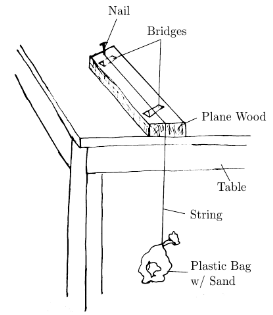
\includegraphics{./img/sonometer.png}
\caption{Construction of a simple sonometer}
\label{fig:sonometert}
\end{center}
\end{figure}

\subsubsection*{Results and Conclusions}
A higher tone is heard/produced if the distance between the two pegs is reduced. A higher tone is also heard/produced if the mass is increased.  
The tone which is produced by the vibrating string/wire depends on its vibrating length and the tension on the string/wire.

\subsubsection*{Clean Up Procedure}
Remove the mass from the string/wire.

\subsubsection*{Discussion Question}
What do you hear in steps 4 and 5?

\subsubsection*{Notes}
The same activity can be used to show that the frequency of a vibrating tuning fork is inversely proportional to the length of a vibrating sting. It can also show that the frequency of a vibrating tuning fork is directly proportional to the tension in a vibrating string. Using different tuning forks and finding the corresponding length and tabulating the values, a graph of Frequency against Reciprocal length can be drawn and is a straight line passing through the origin. Also, wires of different diameters can be fixed on the plane wood. Collect the plane wood, nails from a nearby carpenter and it cost about Tsh.  3, 000/=. Instead of heavy stones, dry sand packed in plastic bags can be used. Also, instead of two pegs you can use two pencils.  
	
	
	%Resonance
	
\subsection{Determination of Resonance Frequency}

\subsubsection*{Learning Objectives}
\begin{itemize}
\item{To explain the concept of resonance as applied to sound} 
\end{itemize}

\subsubsection*{Background Information}
Every object has a natural frequency depending on its size, shape, material, etc.  If a wave drives the object at its natural frequency, the object itself will begin to vibrate along with the wave.  This effect is called resonance.

\subsubsection*{Materials}
Fluorescent tube (tube light), thick rubber tubing, two 1.5 litre plastic water bottles, super glue, wax, turning Fork, retort stand, bucket, water, long stick, knife, metre rule, rubber or cork, piece of cloth

\subsubsection*{Hazards and Safety}
\begin{itemize}
\item{Precautions should be taken when cutting the pipe as it will be sharp.}
\item{Do not touch the fluorescent dust in the tube; it is poisonous.} 
\item{Use glue carefully, do not touch it with you bare fingers.} 
\end{itemize}

\subsubsection*{Preparation Procedure}
\begin{enumerate}
\item{Create a hollow tube from the fluorescent tube by cutting its rims off on both sides.} 
\item{Clean the tube with a piece of cloth attached to a long stick}
\item{Cut the bottom 5 cm off of one of the bottles (bottle 1) and cut the top 5 cm off the top the other bottle (bottle 2).} 
\item{Make a hole in the cap of both bottles.} 
\item{Attach one end of the pipe with the glue and wax to the inside top of bottle 2. Insert the rubber tubing through the holes of both bottle caps.} 
\item{Hold the tube with retort stand together with a metre rule upright(vertically)}
\item{Raise bottle 1 vertically until you have created a U-shape.} 
\item{Pour water into bottle 1.} 
\end{enumerate}

\begin{figure}
\begin{center}
%\def\svgwidth{200pt}
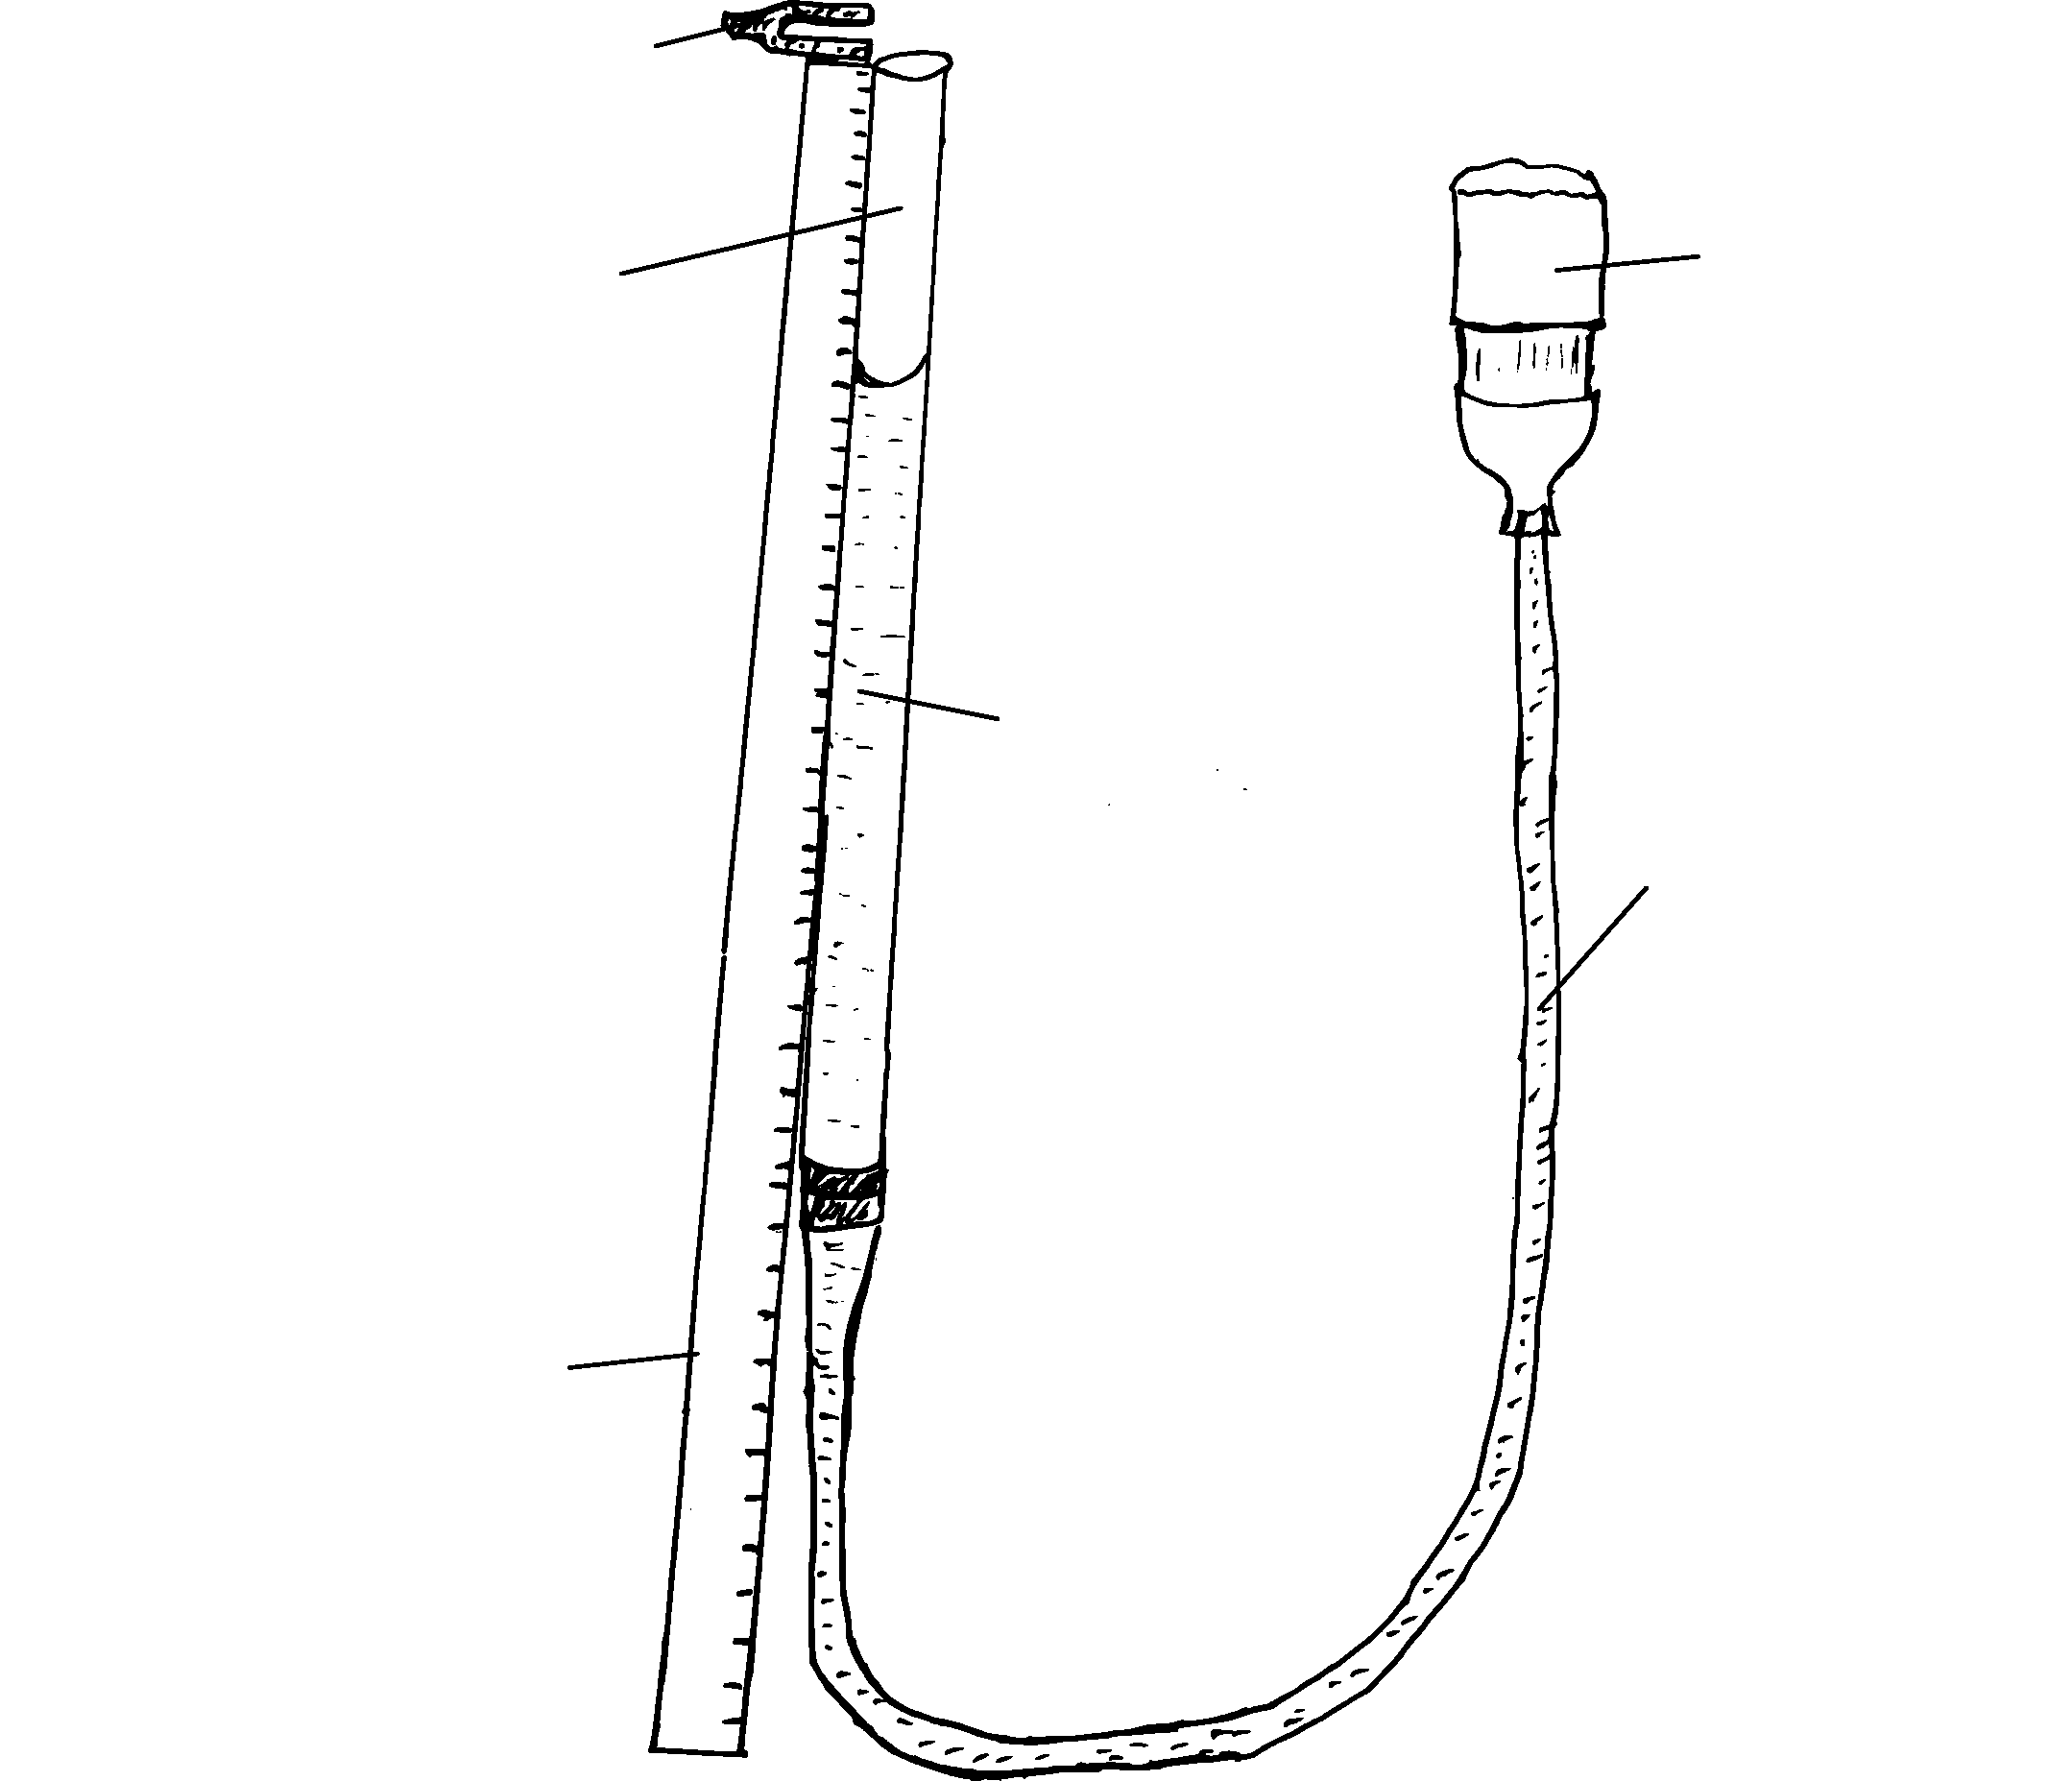
\includegraphics{./img/resonance-tube.png}
\caption{Construction of a resonance tube}
\label{fig:resonance-tube}
\end{center}
\end{figure}

\subsubsection*{Activity Procedure}
\begin{enumerate}
\item{Strike the turning fork with the soft material such as rubber}
\item{Place the turning fork at the top of the tube}
\item{rise and lower the water level in the tube by changing the vertical position of bottle 1}
\item{Repeat for the other two more different turning fork}
\item{For each turning fork note the fundamental note and overtone.} 
\end{enumerate}

\subsubsection*{Results and Conclusions}
Student should hear the tube resonating at two or more water levels. The lowest water level is the fundamental and each smaller water level are higher harmonics.  
Student should understand that: 
The length of the tube from the water to the top can be used to calculate speed of sound in air. 
Resonance frequency occurs when the natural frequency of the air column is equal to the forced frequency from the tuning fork.  

\subsubsection*{Clean Up Procedure}
\begin{enumerate}
\item{Water from the pipe and reservoir pour in the bucket}
\item{Keep the system on the shelves}
\end{enumerate}

\subsubsection*{Discussion Questions}
\begin{enumerate}
\item{Design another way to perform the same experiment.} 
\item{Think of material that can be used instead of fluorescent tube and flexible pipe}
\end{enumerate}

\subsubsection*{Notes}
The vibrating air column in the pipe produces a loud sound when the node of a waveform is at a closed end and the anti-node at the open end. At this point the vibrating air is at resonance with the vibrating tuning fork is held at the open end. 
Teacher should also know that: 
This experience can be used to determine the velocity of sound in air. In absence of the listed materials using the tub in a bucket of water will also work. 
	
	
%Electromagnetic Spectrum (Radio, microwaves, infrared, visible, UV, Xrays, Gamma)


